\documentclass[10pt]{beamer}
% \documentclass[handout,10pt]{beamer}
\usepackage{my_style}
%%%%%%%%%%%%%%%%%%%%%%%%%%%%%%%%%%%%%%%%%%%%%%%%%%%%%%%%%%%%%%%%%%%%%%%%

\title[Math/CS 375]{Lecture 10 - B}
\subtitle{\S 6.1, 6.2 Constructing Quadratic and Cubic Splines}

\begin{document}
% -------------------------------------------------
\begin{frame}
  \titlepage
\end{frame}
% -------------------------------------------------
\begin{frame}{Goals}
We will answer these questions:\\[3mm]
\begin{itemize}
    \item How do you construct a quadratic spline?
    \item What is a cubic spline? 
    \item Is the cubic spline unique?
    \item How do you construct a natural cubic spline?
\end{itemize}
\end{frame}

%%%%%%%%%%%%%%%%%%%%%%%%%%%%%%%%%%%%%%%%%%%%%%%%%%%%%%%%%%%%%%%%%%%%%%%%
\begin{frame}{Spline Interpolation}
\method{Spline Interpolation}{Set of points $(t_i,y_i)$, Degree of smoothness $d$}{Continuous piecewise polynomial $S(x)$}{ Splines interpolate data and do not suffer from large fluctuations between data points. The user controls the smoothness of the interpolation.}
\vspace{3mm}
\begin{itemize}
  \item User controls degree of smoothness
  \begin{itemize}
      \item $d=1$: connect the dots 
      \item $d=2$: piecewise parabolas 
      \item $d=3$: piecewise cubics\\[3mm] 
  \end{itemize}
  \item Example: $d=2 \qquad$
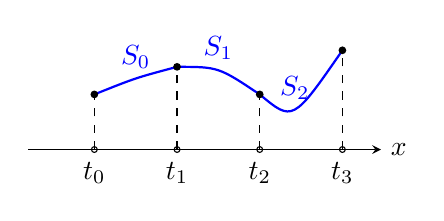
\begin{tikzpicture}[scale=0.7,>=stealth]
% Axis
\draw[->] (-1.2,0) -- (5.2,0) node[right] {$x$};
% Knot positions
\foreach \x/\label in {0/t_0,1.5/t_1,3/t_2,4.5/t_3} {
    \draw (\x,0) circle (1.5pt);
    \node[below] at (\x,-0.05) {$\label$};
}
% Data points
\coordinate (P0) at (0,1.0);
\coordinate (P1) at (1.5,1.5);
\coordinate (P2) at (3.0,1.0);
\coordinate (P3) at (4.5,1.8);
% Vertical dashed lines
\foreach \p in {P0,P1,P2,P3} {
    \draw[dashed] (\p |- 0,0) -- (\p);
}
% Quadratic spline segments (schematic curves)
\draw[thick,blue]
    (P0) .. controls (0.75,1.3) .. (P1)
    node[midway,above] {$S_0$};

\draw[thick,blue]
    (P1) .. controls (2.25,1.5) .. (P2)
    node[midway,above] {$S_1$};

\draw[thick,blue]
    (P2) .. controls (3.6,0.5) .. (P3)
    node[midway,above] {$S_2$};
% Data points
\foreach \p in {P0,P1,P2,P3} {
    \fill (\p) circle (2pt);
}
\end{tikzpicture}
\end{itemize}

\end{frame}


%%%%%%%%%%%%%%%%%%%%%%%%%%%%%%%%%%%%%%%%%%%%%%%%%%%%%%%%%%%%%%%%%%%%%%%%
\sectionframe{Constructing Degree 2 Splines}
%%%%%%%%%%%%%%%%%%%%%%%%%%%%%%%%%%%%%%%%%%%%%%%%%%%%%%%%%%%%%%%%%%%%%%%%


%%%%%%%%%%%%%%%%%%%%%%%%%%%%%%%%%%%%%%%%%%%%%%%%%%%%%%%%%%%%%%%%%%%%%%%%
\begin{frame}{Constructing a Degree 2 Spline}
\begin{center}
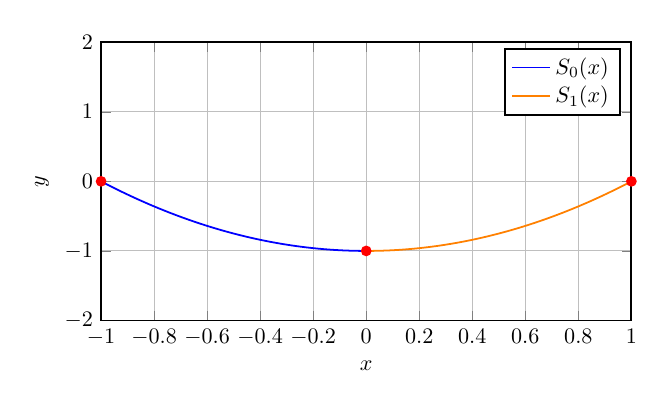
\begin{tikzpicture}[scale=0.8]
    \begin{axis}[
        width=10cm, height=6cm,
        xlabel={$x$}, ylabel={$y$},
        grid=major, 
        thick,
        xmin=-1, xmax=1,
        ymin=-2, ymax=2,
        samples=100,
    ]
    % Quadratic spline segment s0(x) for [-1, 0]
    \addplot[color=blue, thick, domain=-1:0] {x^2-1}; % Example function for s0(x)
    % Quadratic spline segment s1(x) for [0, 1]
    \addplot[color=orange, thick, domain=0:1] {x^2 -1}; % Example function for s1(x)
    % Data points
    \addplot[color=red, only marks, mark=*] 
        coordinates {(-1, 0) (0, -1) (1, 0)};
            \legend{$S_0(x)$, $S_1(x)$};
    \end{axis}
\end{tikzpicture}

\end{center}
\begin{itemize}
    \item Constructing a spline means finding all \textbf{6} unknown coefficients in 
    \begin{align*}
    S_0(x) &= ax^2 + bx+c\\
    S_1(x) & = dx^2 + ex+f
    \end{align*}
    \item We may set up a linear system
\end{itemize}

\end{frame}
%%%%%%%%%%%%%%%%%%%%%%%%%%%%%%%%%%%%%%%%%%%%%%%%%%%%%%%%%%%%%%%%%%%%%%%%
\begin{frame}{Six Conditions}
\begin{block}{Spline Formula}
    \begin{align*}
    S_0(x) &= ax^2 + bx+c\\
    S_1(x) & = dx^2 + ex+f
    \end{align*}
\end{block}
\begin{block}{Conditions}
\begin{enumerate}
    \item $S_0(t_0)=y_0$
    \item $S_0(t_1)=y_1$
    \item $S_1(t_1)=y_1$
    \item $S_1(t_2)=y_2$
    \item $S_0'(t_1)=S_1'(t_1)$
    \item $S_0'(t_0)=0$  \qquad (extra condition)
\end{enumerate}
\end{block}
    
\end{frame}
%%%%%%%%%%%%%%%%%%%%%%%%%%%%%%%%%%%%%%%%%%%%%%%%%%%%%%%%%%%%%%%%%%%%%%%%
\begin{frame}{Apply the Conditions}

\begin{itemize}
    \item Nodes: 
    $$(-1,0) \quad (0,-1),\quad (1,0)$$
    \item Interpolation at endpoints 
    \begin{align*}
    S_0(-1)&=0  &\implies  a -b+c &=0\\ 
    S_0(0)&=-1  &\implies  c &=-1\\
    S_1(0)&=-1  &\implies  f &=-1\\
    S_1(1)&=0   &\implies  d + e + f &=0
    \end{align*}
    \item Smoothness 
    $$
    S_0'(0) = S_1'(0) \implies b = e
    $$
    \item Extra condition 
    $$
    S_0'(-1) = 0 \implies -2a+b = 0
    $$
\end{itemize}

\end{frame}
%%%%%%%%%%%%%%%%%%%%%%%%%%%%%%%%%%%%%%%%%%%%%%%%%%%%%%%%%%%%%%%%%%%%%%%%

\begin{frame}{Linear System}

\begin{itemize}
    \item System 
    $$
    \begin{dcases}
        a - b + c=0\\
        c = -1\\
        f = -1\\
        d + e + f = 0\\
        b -e= 0\\
        -2a+b = 0
    \end{dcases}
    $$
    \item We may write this as
    $$
    \begin{bmatrix}
        1 & -1 & 1 & 0 & 0 &0\\
        0 & 0 & 1 & 0 & 0 & 0\\
        0 & 0 & 0 & 0 & 0 & 1\\
        0 & 0 & 0 & 1 & 1 & 1\\
        0 & 1 & 0 & 0 & -1 & 0\\
        -2 & 1 & 0 & 0 & 0 & 0\\
    \end{bmatrix}\begin{bmatrix}
        a\\b\\c\\d\\e\\f
    \end{bmatrix}=\begin{bmatrix}
        0\\-1\\-1\\0\\0\\0
    \end{bmatrix}
    $$
    \item The solution is
    $$
    x=\begin{bmatrix}
        1 & 0 & -1 & 1 & 0 & -1
    \end{bmatrix}^T$$
\end{itemize}

\end{frame}
%%%%%%%%%%%%%%%%%%%%%%%%%%%%%%%%%%%%%%%%%%%%%%%%%%%%%%%%%%%%%%%%%%%%%%%%
\begin{frame}{Degree 2 Spline}
\begin{center}
    
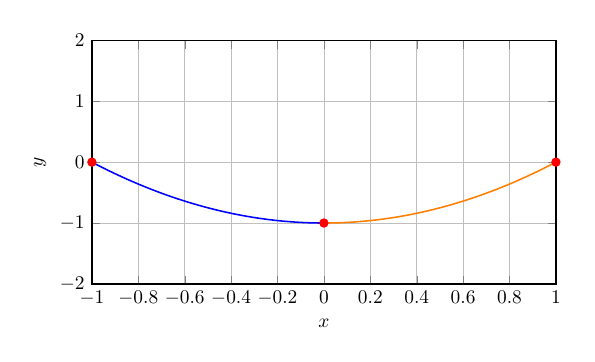
\begin{tikzpicture}[scale=0.7]
    \begin{axis}[
        width=10cm, height=6cm,
        xlabel={$x$}, ylabel={$y$},
        grid=major, 
        thick,
        xmin=-1, xmax=1,
        ymin=-2, ymax=2,
        samples=100,
    ]
    % Quadratic spline segment s0(x) for [-1, 0]
    \addplot[color=blue, thick, domain=-1:0] {x^2-1}; % Example function for s0(x)

    % Quadratic spline segment s1(x) for [0, 1]
    \addplot[color=orange, thick, domain=0:1] {x^2 -1}; % Example function for s1(x)

    % Data points
    \addplot[color=red, only marks, mark=*] 
        coordinates {(-1, 0) (0, -1) (1, 0)};
    \end{axis}
\end{tikzpicture}
\end{center}
\begin{itemize}
    \item Since the solution is
    $$
    x=\begin{bmatrix}
        1 & 0 & -1 & 1 & 0 & -1
    \end{bmatrix}^T$$
    \item The quadratic spline is given by 
    $$
    \begin{dcases}
    x^2 -1, &x\in[-1,0]\\
    x^2 -1, &x\in[0,1]
    \end{dcases}
    $$
\end{itemize}
\end{frame}


%%%%%%%%%%%%%%%%%%%%%%%%%%%%%%%%%%%%%%%%%%%%%%%%%%%%%%%%%%%%%%%%%%%%%%%%
\sectionframe{Bidiagonal System}
%%%%%%%%%%%%%%%%%%%%%%%%%%%%%%%%%%%%%%%%%%%%%%%%%%%%%%%%%%%%%%%%%%%%%%%%

\begin{frame}{Few Problems with the System}
    $$
    \begin{bmatrix}
        1 & -1 & 1 & 0 & 0 &0\\
        0 & 0 & 1 & 0 & 0 & 0\\
        0 & 0 & 0 & 0 & 0 & 1\\
        0 & 0 & 0 & 1 & 1 & 1\\
        0 & 1 & 0 & 0 & -1 & 0\\
        0 & 1 & 0 & 0 & 0 & 0\\
    \end{bmatrix}\begin{bmatrix}
        a_0\\b_0\\c_0\\a_1\\b_1\\c_1
    \end{bmatrix}=\begin{bmatrix}
        0\\-1\\-1\\0\\0\\0
    \end{bmatrix}
    $$
\begin{itemize}
    \item Setting up this system by hand is very awkward
    \item Sparsity pattern is weird
    \item Size is $3n$
\end{itemize}
\vspace{2mm}

\keyidea{
Solving for the coefficients directly is not scalable or structured.
}


\end{frame}

%%%%%%%%%%%%%%%%%%%%%%%%%%%%%%%%%%%%%%%%%%%%%%%%%%%%%
\begin{frame}{A Better Idea}

Instead of solving for coefficients, we change our unknowns.

\bigskip

\begin{block}{New unknowns}
Let
\[
z_i := S'(t_i), \qquad i=0,1,\dots,n
\]
be the slope of the spline at each node.
\end{block}

\begin{itemize}

\item These values describe the \textbf{shape} of the spline

\item The slopes at the nodes can derive the spline pieces $S_i(x)$

\end{itemize}

\keyidea{
Instead of coefficients, we solve for the slopes at the nodes.
}

\end{frame}
%%%%%%%%%%%%%%%%%%%%%%%%%%%%%%%%%%%%%%%%%%%%%%%%%%%%%
\begin{frame}{Reconstructing Each Piece}

On each interval $[t_i,t_{i+1}]$, we want:

\begin{itemize}
\item $S_i(t_i) = y_i$
\item $S_i(t_{i+1}) = y_{i+1}$
\item $S_i'(t_i) = z_i$
% \item $S_i'(t_{i+1}) = z_{i+1}$
\end{itemize}

\bigskip

A quadratic polynomial is uniquely determined by:
\[
\text{value + slope at two points}
\]

\bigskip

\keyidea{
Knowing $y_i,y_{i+1},z_i,z_{i+1}$ determines $S_i(x)$ completely.
}

\end{frame}
%%%%%%%%%%%%%%%%%%%%%%%%%%%%%
\begin{frame}{Mini Example}

\begin{example}
Find a quadratic polynomial of the form
\[
p_2(x)=a(x-1)^2 + b(x-1) + c
\]
such that:
\begin{itemize}
    \item $p_2(1)=2$
    \item $p_2(2)=5$
    \item $p_2'(1)=1$
    % \item $p_2'(2)=3$
\end{itemize}
\end{example}

\pause

\begin{block}{Why this form?}
We center the polynomial at $x=1$ so the conditions at $x=1$
become very simple.
\end{block}

\end{frame}
%%%%%%%%%%%%%%%%%%%%%%%%%%%%%
%%%%%%%%%%%%%%%%%%%%%%%%%%%%%
\begin{frame}{Solving the Example}

\begin{itemize}

\item First compute the derivative:
\[
p_2'(x) = 2a(x-1) + b
\]



\item Apply conditions at $x=1$:
\[
p_2(1)=c=2
\]
\[
p_2'(1)=b=1
\]

\item Now use conditions at $x=2$:
\[
p_2(2)=a(1)^2 + b(1) + c = a + b + c = 5
\]
\[
a + 1 + 2 = 5 \Rightarrow a = 2
\]
\item Result 
$$
    p(x)= 2(x-1)^2 +(x-1)+2
$$


% \item Check derivative:
% \[
% p_2'(2)=2a(1)+b=2(2)+1=5 \;\; \text{(adjust data if needed)}
% \]

\end{itemize}

\end{frame}
%%%%%%%%%%%%%%%%%%%%%%%%%%%%%
\begin{frame}{Constructing $S_i(x)$}

\begin{itemize}


\item Instead of $ S_i(x) = a_i x^2 + b_i x + c_i$, we will let 
    \[
S_i(x)
=
\frac{z_{i+1}-z_i}{2h_i}(x-t_i)^2
+ z_i(x-t_i) + y_i, \quad h_i = t_{i+1}-t_i
\]
\item The derivative is 
    \[
S_i'(x)
=
\frac{z_{i+1}-z_i}{h_i}(x-t_i)
+ z_i
\]
\item Notice that we immediately get 
\begin{itemize}
    \item $S(t_i)=y_i$,
    \item $S'(t_i)=z_i$,
    \item $S'(t_{i+1})=z_{i+1}$.
\end{itemize}
\end{itemize}
% \onslide<2>{
% \question{What about the fourth condition $S_i(t_{i+1}) = y_{i+1} $?}
% }
\end{frame}

\begin{frame}{Equations for $z_i$}
\begin{itemize}
    \item  Since $S(x)$ interpolates $(t_{i+1},y_{i+1})$ we must have 
    $$
        S_i(t_{i+1}) = y_{i+1} 
    $$

\item Substituting $x=t_{i+1}$ into 
\begin{align*}    
S_i(t_{i+1})=&\frac{z_{i+1}-z_i}{2h_i}(t_{i+1}-t_i)^2+ z_i(t_{i+1}-t_i) + y_i\\
=&\frac{z_{i+1}-z_i}{2}h_i+ z_ih_i + y_i=y_{i+1}
\end{align*}
\item With a bit of rearrangement 
\[
z_i+z_{i+1}
=
2\,\frac{y_{i+1}-y_i}{h_i},
\qquad i=0,\dots,n-1.
\]
\end{itemize}
\question{What type of linear system will this equation yield?}
\end{frame}


%%%%%%%%%%%%%%%%%%%%%%%%%%%%%%%%%%%
\begin{frame}[shrink]{The Bidiagonal System}

Explicitly writing out this equation for values of $i\dots$
\[
z_i + z_{i+1}
=
2\,\frac{y_{i+1}-y_i}{h_i} = r_i,
\qquad i=0,\dots,n-1,
\]
\begin{align*}
i=0:\quad & z_0 + z_1 = r_0\\
i=1:\quad & z_1 + z_2 = r_1\\
& \;\;\vdots\\
i=n-1:\quad & z_{n-1} + z_n = r_{n-1}
\end{align*}

\onslide<2>{
In $Ax=b$ form, we get a \textbf{bidiagonal matrix}!
\[
\begin{bmatrix}
1 & 1 &   &   &   \\
  & 1 & 1 &   &   \\
  &   & 1 & 1 &   \\
  &   &   & \ddots & \ddots \\
  &   &   &        & 1 \;\; 1
\end{bmatrix}
\begin{bmatrix}
z_0\\
z_1\\
z_2\\
\vdots\\
z_n
\end{bmatrix}
=
\begin{bmatrix}
r_0\\
r_1\\
r_2\\
\vdots\\
r_{n-1}
\end{bmatrix}
\]
}


\end{frame}
%%%%%%%%%%%%%%%%%%%%%%%%%%%%%%%%%%%

\begin{frame}{Quadratic Spline Algorithm}

\begin{enumerate}
    \item Choose an initial derivative value $z_0 = S'(t_0)$.
    \item Use the recurrence to set up a linear system 
    \[
    z_i + z_{i+1}
      =
    2\,\frac{y_{i+1}-y_i}{t_{i+1}-t_i} =: r_i
    \]
    $$
    \begin{bmatrix}
        1 &1 & & \\
          &1 &1& \\
          & &\ddots&\ddots \\
          & && 1&  1
    \end{bmatrix}\begin{bmatrix}
        z_0\\z_1\\\vdots\\z_n 
    \end{bmatrix} = \begin{bmatrix}
        r_0\\r_1\\\vdots\\r_n
    \end{bmatrix}
    $$
    \item Do back substitution and then compute the spline function with the formula 
        \[
        S_i(x)
        =
        \frac{z_{i+1}-z_i}{2h_i}(x-t_i)^2
        + z_i(x-t_i) + y_i, \quad h_i = t_{i+1}-t_i
        \]
\end{enumerate}
\end{frame}

%%%%%%%%%%%%%%%%%%%%%%%%%%%%%%%%%%%%%%%%%%%%%%%%%%%%%%%%%%%%%%%%%%%%%%%%
\begin{frame}[shrink]{Summary}
\begin{itemize}
    \item A system in terms of the spline coefficients is awkward
        $$
    \begin{bmatrix}
        1 & -1 & 1 & 0 & 0 &0\\
        0 & 0 & 1 & 0 & 0 & 0\\
        0 & 0 & 0 & 0 & 0 & 1\\
        0 & 0 & 0 & 1 & 1 & 1\\
        0 & 1 & 0 & 0 & -1 & 0\\
        0 & 1 & 0 & 0 & 0 & 0\\
    \end{bmatrix}\begin{bmatrix}
        a_0\\b_0\\c_0\\a_1\\b_1\\c_1
    \end{bmatrix}=\begin{bmatrix}
        0\\-1\\-1\\0\\0\\0
    \end{bmatrix}
    $$
    \item A system in terms of  $S'(t_i)=z_i$ is structured 
    $$
    \begin{bmatrix}
        1 &1 & & \\
          &1 &1& \\
          & & 1&    1
    \end{bmatrix}\begin{bmatrix}
        z_0\\z_1\\z_2
    \end{bmatrix} = \begin{bmatrix}
        r_0\\r_1\\r_2
    \end{bmatrix}
    $$
\end{itemize}
\keyidea{
Advantages: 
\begin{itemize}
    \item Systematic
    \item Smaller linear system 
    \item Fast $\mO(n)$ solve
\end{itemize}
}
\end{frame}


%%%%%%%%%%%%%%%%%%%%%%%%%%%%%%%%%%%%%%%%%%%%%%%%%%%%%%%%%%%%%%%%%%%%%%%%
\sectionframe{Cubic Spline}
%%%%%%%%%%%%%%%%%%%%%%%%%%%%%%%%%%%%%%%%%%%%%%%%%%%%%%%%%%%%%%%%%%%%%%%%
\begin{frame}{Third-Degree Spline or Cubic Spline}
\define{Degree Three Spline}{
A function $S(x)$ is a \textbf{spline of degree 3} if:
\begin{enumerate}
  \item The domain of $S(x)$ is an interval $[a,b]$
  \item $S(x)$ is continuous on $[a,b]$
  \item $S'(x)$ is continuous on $[a,b]$
  \item $S''(x)$ is continuous on $[a,b]$
  \item There is a partition $a=t_0<t_1<\dots<t_n=b$ such that $S(x)$ is
cubic on each subinterval $[t_i,t_{i+1}]$.
\end{enumerate}
}

% \vspace{4mm}
% \question{
% Is the construction of a cubic spline a well-defined problem?
% }
\vfill
Two differences from \textbf{degree two} splines:
\begin{itemize}
    \item Condition 4: $S''(x)$ is continuous 
    \item Condition 5: Each spline piece is cubic 
\end{itemize}
\end{frame}

%%%%%%%%%%%%%%%%%%%%%%%%%%%%%%%%%%%%%%%%%%%%%%%%%%%%%%%%%%%%%%%%%%%%%%
\begin{frame}{Smoothness Condition}
\begin{center}
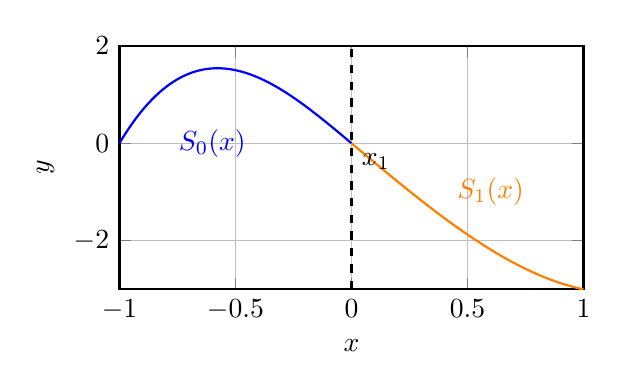
\begin{tikzpicture}
\begin{axis}[
    scale=0.7,
    width=10cm, height=6cm,
    xlabel={$x$}, ylabel={$y$},
    grid=major, 
    thick,
    xmin=-1, xmax=1,
    ymin=-3, ymax=2,
    samples=100,
    clip=false
]

% Left spline S0
\addplot[color=blue, thick, domain=-1:0] {4*(x-1)*x*(x+1)};
\node[blue,above] at (axis cs:-0.6,-0.5) {$S_0(x)$};

% Right spline S1
\addplot[color=orange, thick, domain=0:1] {(x-2)*x*(x+2)};
\node[orange,below] at (axis cs:0.6,-0.5) {$S_1(x)$};


% Label nodes
\node[below right] at (0,0) {$x_1$};


% Highlight the junction
\draw[dashed] (axis cs:0,-3) -- (axis cs:0,2);
% \node[above] at (axis cs:0,1.5) {\small junction};

% Indicate matching slope
% \draw[->, thick] (axis cs:-0.15,-1.2) -- (axis cs:0,-1);
% \draw[->, thick] (axis cs:0.15,-1.2) -- (axis cs:0,-1);

% \node at (axis cs:0,-1.5) {\small matching slope};

\end{axis}
\end{tikzpicture}
\end{center}

\begin{itemize}
    \item For continuity of $S'(x)$ we need 
    $$
        S_0'(x_1) = S_1'(x_1)
    $$
    \item For continuity of $S''(x)$ we need 
    $$
        S_0''(x_1) = S_1''(x_1)
    $$
\end{itemize}

\end{frame}

%%%%%%%%%%%%%%%%%%%%%%%%%%%%%%%%%%%%%%%%%%%%%%%%%%%%%%%%%%%%%%%%%%%%%%
\begin{frame}{Number of Unknowns}

{
\question{If there are $n+1$ data points, how many unknowns does a cubic spline have?}
}

\begin{itemize}
\item  Each component of $S(x)$ has the form
\begin{equation*}
  S_i(x) = ax^3 + bx^2 + cx + d
\end{equation*}
\vfill 
\item Cubics have \textbf{4 unknown coefficients} per subinterval 
\vfill 
\item $n+1$ data points $\implies$ $n$ subintervals
\vfill
\begin{block}{Number of Unknown Coefficients}
A cubic spline has
$$ \textbf{4n total unknowns}$$
\end{block}
\vfill
\end{itemize}
\end{frame}
%%%%%%%%%%%%%%%%%%%%%%%%%%%%%%%%%%%%%%%%%%%%%%%%%%%%%%%%%%%%%%%%%%%%%%%%
\begin{frame}{Number of Constraints}

% \begin{center}
% \begin{tikzpicture}[scale=0.5,>=stealth]
% % Axis
% \draw[->] (-1.2,0) -- (5.2,0) node[right] {$x$};
% % Knot positions
% \foreach \x/\label in {0/t_0,1.5/t_1,3/t_2,4.5/t_3} {
%     \draw (\x,0) circle (1.5pt);
%     \node[below] at (\x,-0.05) {$\label$};
% }
% \foreach \x/\label in {1.5/t_1,3/t_2} {
%     \draw (\x,0) circle (1.5pt);
%     \node[below] at (\x,-0.05) {\red{$\label$}};
% }
% % ---- Brace for interior nodes ----
% \draw[decorate,decoration={brace,mirror,amplitude=6pt}]
%   (1.3,-0.70) -- (3.2,-0.7)
%   node[midway,below=8pt] {interior nodes};

% % Data points
% \coordinate (P0) at (0,1.0);
% \coordinate (P1) at (1.5,1.5);
% \coordinate (P2) at (3.0,1.0);
% \coordinate (P3) at (4.5,1.8);
% % Vertical dashed lines
% \foreach \p in {P0,P1,P2,P3} {
%     \draw[dashed] (\p |- 0,0) -- (\p);
% }
% % Quadratic spline segments (schematic curves)
% \draw[thick,blue]
%     (P0) .. controls (0.75,1.3) .. (P1)
%     node[midway,above] {$S_0$};

% \draw[thick,blue]
%     (P1) .. controls (2.25,1.5) .. (P2)
%     node[midway,above] {$S_1$};

% \draw[thick,blue]
%     (P2) .. controls (3.6,0.5) .. (P3)
%     node[midway,above] {$S_2$};
% % Data points
% \foreach \p in {P0,P1,P2,P3} {
%     \fill (\p) circle (2pt);
% }
% \end{tikzpicture}
% \end{center}

\begin{itemize}
    \item Interpolation at the endpoints $S_i(t_i)=y_i$ and $S_i(t_{i+1})=y_{i+1}$ so
    $$ \textbf{2n constraints}$$
    \item We need continuous 1st order derivative $S_i'=S_{i+1}'$ at interior nodes so 
    $$\textbf{n-1 constraints}$$
    \item We need continuous 2nd order derivative $S_i''=S_{i+1}''$ at interior nodes so 
    $$\textbf{n-1 constraints}$$
\begin{block}{Number of Unknown Coefficients}
A general cubic spline with $n+1$ nodes has 
    $$\textbf{4n-2 total constraints}$$
\end{block}
\end{itemize}
    
\end{frame}

%%%%%%%%%%%%%%%%%%%%%%%%%%%%%%%%%%%%%%%%%%%%%%%%%%%%%%%%%%%%%%%%%%%%%%%%
\begin{frame}{Uniqueness for Cubic Splines}

\begin{block}{Underdetermined}
$$\textbf{4n unknowns}\quad vs.\quad \textbf{4n-2 constraints}$$
\end{block}

Common options to fill two missing constraints:\\[3mm]
  \begin{itemize}
    \item \textbf{Natural}: $S''(t_0)=S''(t_n)=0$ \bigskip 
    \item \textbf{Clamped}: $S'(t_0)=a$, $S'(t_n)=b$ \bigskip
    %\item not-a-knot: $S'''(x)$ continuous at $t_1$ and $t_{n-1}$
    \item \textbf{Periodic}: $S'$ and $S''$ are periodic at the ends\\
       $S'(t_0) = S'(t_n)$ and $S''(t_0) = S''(t_n)$
  \end{itemize}
\vspace{4mm}
\keyidea{
\begin{itemize}
    \item A generic cubic spline is \textbf{NOT} unique
    \item Cubic splines are\textbf{ missing two constraints} 
    \item A common choice to use include natural conditions 
\end{itemize}
}

\end{frame}

%%%%%%%%%%%%%%%%%%%%%%%%%%%%%%%%%%%%%%%%%%%%%%%%%%%%%%%%%%%%%%%%%%%%%%%%
\sectionframe{Tridiagonal System}
%%%%%%%%%%%%%%%%%%%%%%%%%%%%%%%%%%%%%%%%%%%%%%%%%%%%%%%%%%%%%%%%%%%%%%%%
% \begin{frame}{Consider solving for the coefficients}

% \begin{itemize}
%     \item How do you find the natural cubic spline for
% \begin{tabular}{c | c c c }
% $x$ & -1 & 0 & 1\\\hline
% $y$ & 1 & 2 & -1\\
% \end{tabular} ? 


% \item We can write out our unknowns as $c$
% \begin{align*}
%     S_0(x) &= c_{1} + c_{2} x + c_{3} x^2 + c_{4} x^3\\
%     S_1(x) &= c_{5} + b_6 x + c_7 x^2 + c_8 x^3
% \end{align*}

% \item We can write out 8 conditions to set up a linear system 
%     $$ A c = g$$
% since its a square system. But the system is a bit awkward. 

% \begin{block}{Idea}
% \begin{itemize}
%     \item Instead of $Ac=g$,  we set up an alternative tridiagonal system $Hz = v$. 
%     \item The next few slides explain the steps to construct the system.
% \end{itemize}
% \end{block}
    
% \end{itemize}

% \end{frame}

%%%%%%%%%%%%%%%%%%%%%%%%%%%%%%%%%%%%%%%%%%%%%%%%%%%%%%%%%%%%%%%%%%%%%%%%
\begin{frame}{Goal}

\begin{block}{Problem}
\begin{itemize}
    \item Given $n+1$ data points $(t_i, y_i)$ for $i=0$ to $n$
    \item Assume natural conditions $S''(t_0) = S''(t_n)=0$
    \item Construct the cubic spline 
\end{itemize}
\end{block}

\begin{block}{The Idea}
    \begin{itemize}
\item Instead of $S_i(x)= a_ix^3 + b_ix^2 + c_ix + d_i$, let 
    \begin{equation*}
      S_i(x) = \frac{z_i}{6h_i}(t_{i+1}-x)^3 +\frac{z_{i+1}}{6h_i}(x-t_i)^3 + C_i(x-t_i) + D_i(t_{i+1}-x),
    \end{equation*}

\item Set up a linear system for $z_i=S''(t_i)$
\end{itemize}
\end{block}
    
\end{frame}
%%%%%%%%%%%%%%%%%%%%%%%%%%%%%%%%%%%%%%%%%%%%%%%%%%%%%%%%%%%%%%%%%%%%%%%%

\begin{frame}{Natural Cubic Spline: Step 1}

\begin{itemize}
\item Notice the formula
    \begin{equation*}
      S_i(x) = \underbrace{\frac{z_i}{6h_i}(t_{i+1}-x)^3 +\frac{z_{i+1}}{6h_i}(x-t_i)^3}_{\text{two cubics}} + \underbrace{C_i(x-t_i) + D_i(t_{i+1}-x)}_{\text{two linears}}
    \end{equation*}
  
\item First derivative 
$$
    S_i'(x) = -\frac{z_i}{2h_i}(t_{i+1}-x)^2 +\frac{z_{i+1}}{2h_i}(x-t_i)^2 + C_i -D_i
$$
\item Second derivative
$$
    S_i''(x) = \frac{z_i}{h_i}(t_{i+1}-x) +\frac{z_{i+1}}{h_i}(x-t_i) 
$$
\end{itemize}
   
\end{frame}
%%%%%%%%%%%%%%%%%%%%%%%%%%%%%%%%%%%%%%%%%%%%%%%%%%%%%
\begin{frame}{Natural Cubic Spline: Step 2}

\begin{itemize}
\item We require these six conditions on the spline
\begin{enumerate}
    \item $S_i(t_i)=y_i$
    \item $S_i(t_{i+1})=y_{i+1}$
    \item $S_i'(t_{i})=S'_{i-1}(t_i)$
    \item $S_i'(t_{i+1})=S'_{i+1}(t_{i+1})$
    \item $S_i''(t_{i})=z_i$
    \item $S_i''(t_{i+1})=z_{i+1}$
\end{enumerate}
\vfill
    \item Since $S_i''(x) = \frac{z_i}{h_i}(t_{i+1}-x) +\frac{z_{i+1}}{h_i}(x-t_i)$ we immediately have 
    \begin{itemize}
            \item Condition 5: $S_i''(t_{i})=z_i$
    \item Condition 6: $S_i''(t_{i+1})=z_{i+1}$
    \end{itemize}
    \vfill 
    \item Now we enforce the other 4 conditions
\end{itemize}
   
\end{frame}

%%%%%%%%%%%%%%%%%%%%%%%%%%%%%%%%%%%%%%%%%%%%%%%%%%%%%%%%%%%%%%%%%%%%%%%%
\begin{frame}{Natural Cubic Spline: Step 3}
         $$ S_i(x) = \frac{z_i}{6h_i}(t_{i+1}-x)^3 +\frac{z_{i+1}}{6h_i}(x-t_i)^3 + C_i(x-t_i) + D_i(t_{i+1}-x) $$

\begin{itemize}
    \item Apply Condition 1:  $S_i(t_i)=y_i$ to get a formula for $D_i$
        \begin{align*}
          y_i & = S_i(t_i) = \frac{z_i}{6h_i}(t_{i+1}-t_i)^3    + D_i(t_{i+1}-t_i)\\
              & = \frac{z_i}{6}h_i^2 + D_i h_i\\
         \therefore\quad D_i & = \frac{y_i}{h_i} - \frac{h_i}{6}z_i 
        \end{align*}
    \item Apply Condition 2: $S_i(t_{i+1})=y_{i+1}$ to get a formula for $C_i$
        \begin{align*}
          y_{i+1} & = S_i(t_{i+1}) =   \frac{z_{i+1}}{6h_i}(t_{i+1}-t_i)^3 + C_i(t_{i+1}-t_i)  \\
          & = \frac{z_{i+1}}{6}(h_i)^2 + C_ih_i\\
         \therefore\quad C_i & = \frac{y_{i+1}}{h_i} - \frac{h_i}{6}z_{i+1}
        \end{align*}
\end{itemize}
\end{frame}

%%%%%%%%%%%%%%%%%%%%%%%%%%%%%%%%%%%%%%%%%%%%%%%%%%%%%%%%%%%%%%%%%%%%%%%%
\begin{frame}[shrink]{Natural Cubic Spline: Step 3}
\vspace{-10pt}

\begin{equation*}
  S_i(x) = \frac{z_i}{6h_i}(t_{i+1}-x)^3
+\frac{z_{i+1}}{6h_i}(x-t_i)^3 
+\left(\frac{y_{i+1}}{h_i} - \frac{h_i}{6}z_{i+1}\right)(x-t_i)
+\left(\frac{y_i}{h_i} - \frac{h_i}{6}z_i\right) (t_{i+1}-x)
\end{equation*}\vspace{-1pt}

\begin{itemize}
    \item We know the derivatives
        \begin{align*}
          S'_i(x) &= -\frac{z_i}{2h_i}(t_{i+1}-x)^2 +\frac{z_{i+1}}{2h_i}(x-t_i)^2 + C_i-D_i\\
          S'_{i-1}(x) &= -\frac{z_{i-1}}{2h_i}(t_{i}-x)^2 +\frac{z_{i}}{2h_{i-1}}(x-t_{i-1})^2 + C_{i-1}-D_{i-1}\\
        \end{align*} 

\item Apply Condition 3: $S'_i(t_i) = S'_{i-1}(t_i)$: \vspace{-3pt}
    \begin{align*}
      S'_i(t_i) &= -\frac{h_i}{6}z_{i+1}  +C_i-D_i\\
      S'_{i-1}(t_i) &= \frac{h_{i-1}}{6}z_{i} + C_{i-1}-D_{i-1}
    \end{align*}
\item We have 
$$
-\frac{h_i}{6}z_{i+1}  +C_i-D_i = \frac{h_{i-1}}{6}z_{i} + C_{i-1}-D_{i-1}
$$
\end{itemize}
\end{frame}
%%%%%%%%%%%%%%%%%%%%%%%%%%%%%%%%%%%%%%%%%%%%%%%%%%%%%%%%%%%%%%%%%%%%%%%%
\begin{frame}{Natural Cubic Spline: Step 4}
\begin{itemize}

\item Substitute $C_i, D_i$ and simplify each side

\item Left-hand side:
\begin{align*}
-\frac{h_i}{6}z_{i+1} + C_i - D_i
&= -\frac{h_i}{6}z_{i+1}
+ \left(\frac{y_{i+1}}{h_i} - \frac{h_i}{6}z_{i+1}\right)
- \left(\frac{y_i}{h_i} - \frac{h_i}{6}z_i\right) \\
&= \frac{y_{i+1}-y_i}{h_i}
- \frac{h_i}{3}z_{i+1}
+ \frac{h_i}{6}z_i
\end{align*}

\item Right-hand side:
\begin{align*}
\frac{h_{i-1}}{6}z_i + C_{i-1} - D_{i-1}
&= \frac{h_{i-1}}{6}z_i
+ \left(\frac{y_i}{h_{i-1}} - \frac{h_{i-1}}{6}z_i\right)
- \left(\frac{y_{i-1}}{h_{i-1}} - \frac{h_{i-1}}{6}z_{i-1}\right) \\
&= \frac{y_i - y_{i-1}}{h_{i-1}}
+ \frac{h_{i-1}}{6}z_{i-1}
- \frac{h_{i-1}}{3}z_i
\end{align*}

\end{itemize}
\end{frame}

%%%%%%%%%%%%%%%%%%%%%%%%%%%%%%%%%%%%%%%%%%%%%%%%%%%%%%%%%%%%%%%%%%%%%%%%
\begin{frame}{Natural Cubic Spline: Step 5}
\begin{itemize}

\item The simplified form of $S'_i(t_i) = S'_{i-1}(t_i)$ is:
\begin{align*}
\frac{y_{i+1}-y_i}{h_i}
- \frac{h_i}{3}z_{i+1}
+ \frac{h_i}{6}z_i
=
\frac{y_i - y_{i-1}}{h_{i-1}}
+ \frac{h_{i-1}}{6}z_{i-1}
- \frac{h_{i-1}}{3}z_i
\end{align*}

\item Rearranging gives the final equation:

\begin{block}{Formula for $z$'s}
\begin{equation*}
h_{i-1}z_{i-1} + 2(h_i+h_{i-1})z_i + h_i z_{i+1}
= 6(b_i - b_{i-1}),
\end{equation*}
\[
b_i = \frac{y_{i+1}-y_i}{h_i}
\]
\end{block}

\end{itemize}
\end{frame}
%%%%%%%%%%%%%%%%%%%%%%%%%%%%%%%%%%%%%%%%%%%%%%%%%%%%%%%%%%%%%%%%%%%%%%%%

\begin{frame}{Tridiagonal System}

\begin{itemize}
    \item This is a recurrence equation
\[
h_{i-1}z_{i-1} + 2(h_i+h_{i-1})z_i + h_i z_{i+1}
= 6(b_i - b_{i-1}), \quad i=1,\dots,n-1,
\]

\item Substituting for a few values of $i\dots$

\begin{align*}
i=1:\quad & h_0 z_0 + 2(h_1+h_0)z_1 + h_1 z_2 = 6(b_1 - b_0)\\
i=2:\quad & h_1 z_1 + 2(h_2+h_1)z_2 + h_2 z_3 = 6(b_2 - b_1)\\
i=3:\quad & h_2 z_2 + 2(h_3+h_2)z_3 + h_3 z_4 = 6(b_3 - b_2)\\
& \;\;\vdots\\
i=n-1:\quad & h_{n-2} z_{n-2} + 2(h_{n-1}+h_{n-2})z_{n-1} + h_{n-1} z_n
= 6(b_{n-1} - b_{n-2})
\end{align*}

\end{itemize}

\begin{block}{Observation}
Each equation involves only three neighboring unknowns:
\[
z_{i-1}, \quad z_i, \quad z_{i+1}.
\]
\end{block}


\end{frame}
%%%%%%%%%%%%%%%%%%%%%%%%%%%%%%%%%%%%%%%%%%%%%%%%%%%%%%%%%%%%%%%%%%%%%%%%

\begin{frame}{Natural Cubic Spline: Summary}
The $z_i$ are defined by
\begin{equation*}
  h_{i-1}\red{z_{i-1}} + 2(h_i+h_{i-1})\red{z_i} + h_{i}\red{z_{i+1}} = 6(b_i-b_{i-1}) =: v_i
\end{equation*}
   \vspace{-10pt}
\begin{itemize}
  \item For natural conditions $z_0=z_n=0$, from $S''(t_0)=S''(t_n)=0$ 
  \item Set up a \textbf{tridiagonal linear system} and solve it in $\mO(n)$ FLOPs
\end{itemize}
\[
\begin{bmatrix}
 1 &  & & & & & & \\ 
 h_0 & u_1  & h_1 & & & & & \\ 
 & h_1            &  u_2 & h_2 & & & & \\ 
 &                & h_2             & u_3 & h_3  & & & \\ 
 &                &                 & \ddots  & \ddots & \ddots & & \\  
 &  &   &   & h_{n-3} & u_{n-2} & h_{n-2}  & \\ 
 &  &   &   &         & h_{n-2} &  u_{n-1}& h_{n-1}\\
 &  &   &   &         &         &        & 1\\
\end{bmatrix}
\begin{bmatrix}
z_0\\z_1\\  z_2\\  z_3\\  \vdots\\  z_{n-2}\\  z_{n-1}\\z_n\\
\end{bmatrix}
 = 
\begin{bmatrix}
0\\v_1\\  v_2\\  v_3\\  \vdots\\  v_{n-2}\\  v_{n-1}\\0\\
\end{bmatrix}
\] 
\begin{eqnarray*}
u_i & = & 2 (h_i + h_{i-1} ) \\
v_i & = & 6(b_i - b_{i-1})
\end{eqnarray*} 
\end{frame}

%%%%%%%%%%%%%%%%%%%%%%%%%%%%%%%%%%%%%%%%%%%%%%%%%%%%%%%%%%%%%%%%%%%%%%%%
\begin{frame}{Natural Cubic Spline: Conclusion}

\begin{enumerate}
    \item Calculate $h_i=t_{i+1}-t_i$, $b_i=\frac{1}{h_i}(y_{i+1}-y_i)$,$u_i = 2 (h_i + h_{i-1} )$, and $v_i = 6(b_i - b_{i-1})$

    \item Set up the tridiagonal system 
    \[
\begin{bmatrix}
 1 &  & & &  \\ 
 h_0 & u_1  & h_1 & &  \\ 
 &   \ddots  & \ddots & \ddots  \\  
 &  & h_{n-2} &  u_{n-1}& h_{n-1}\\
 &  &   &         & 1\\
\end{bmatrix}
\begin{bmatrix}
z_0\\z_1\\  \vdots\\  z_{n-1}\\z_n\\
\end{bmatrix}
 = 
\begin{bmatrix}
0\\v_1\\  \vdots\\   v_{n-1}\\0\\
\end{bmatrix}
\] 

    \item Solve the system

    \item Construct the spline function
\begin{equation*}
  S_i(x) = \frac{z_i}{6h_i}(t_{i+1}-x)^3
+\frac{z_{i+1}}{6h_i}(x-t_i)^3 + C_i(x-t_i) + D_i(t_{i+1}-x)
\end{equation*}
where
\begin{equation*}
  D_i = \frac{y_i}{h_i} - \frac{h_i}{6}z_i \qquad
  C_i = \frac{y_{i+1}}{h_i} - \frac{h_i}{6}z_{i+1}
\end{equation*}
\end{enumerate}
\end{frame}


%%%%%%%%%%%%%%%%%%%%%%%%%%%%%%%%%%%%%%%%%%%%%%%%%%%%%%%%%%%%%%%%%%%%%%%%
\begin{frame}{Algorithm: page 269 NMC7 (page 391, NMC6)}
In practice, you do not actually construct a tridiagonal system and solve it (though it is more convenient). It is more efficient to directly solve for  $z_i$ in a loop. \bigskip

See algorithm in the book for efficient implementation. \bigskip 

\begin{enumerate}
  \item Compute for $i=0,\dots,n-1$
  \begin{equation*}
  h_i=t_{i+1}-t_i\qquad b_i=\frac{1}{h_i}(y_{i+1}-y_{i})
  \end{equation*}
  \item Set $u$, $v$:
  \item Tridiagonal solve to get $z$
  \item Substitute into the nested form for $S(x)$ equation 12, page 270 NMC7 (NMC6: equation 12 page 392)
\end{enumerate}
\end{frame}
%%%%%%%%%%%%%%%%%%%%%%%%%%%%%%%%%%%%%%%%%%%%%%%%%%%%%%%%%%%%%%%%%%%%%%%
\begin{frame}{Main Point}
    \begin{itemize}
        \item Suppose you are given $n+1$ data points $(t_i,y_i)$

        \item Then constructing the natural cubic spline amounts to solving 
        \[
\begin{bmatrix}
 1 &  & & & & & & \\ 
 h_0 & u_1  & h_1 & & & & & \\ 
 & h_1            &  u_2 & h_2 & & & & \\ 
 &                & h_2             & u_3 & h_3  & & & \\ 
 &                &                 & \ddots  & \ddots & \ddots & & \\  
 &  &   &   & h_{n-3} & u_{n-2} & h_{n-2}  & \\ 
 &  &   &   &         & h_{n-2} &  u_{n-1}& h_{n-1}\\
 &  &   &   &         &         &        & 1\\
\end{bmatrix}
\begin{bmatrix}
z_0\\z_1\\  z_2\\  z_3\\  \vdots\\  z_{n-2}\\  z_{n-1}\\z_n\\
\end{bmatrix}
 = 
\begin{bmatrix}
0\\v_1\\  v_2\\  v_3\\  \vdots\\  v_{n-2}\\  v_{n-1}\\0\\
\end{bmatrix}
\] 
    \keyidea{This is a tridiagonal system. Finding the natural cubic spline only costs $\mO(n)$ FLOPs.}
    \end{itemize}
\end{frame}
%%%%%%%%%%%%%%%%%%%%%%%%%%%%%%%%%%%%%%%%%%%%%%%%%%%%%%%%%%%%%%%%%%%%%%%
\begin{frame}{Runge's Phenomenon}

\begin{block}{Example - Try interpolation on this data set}
\begin{figure}
    \centering
    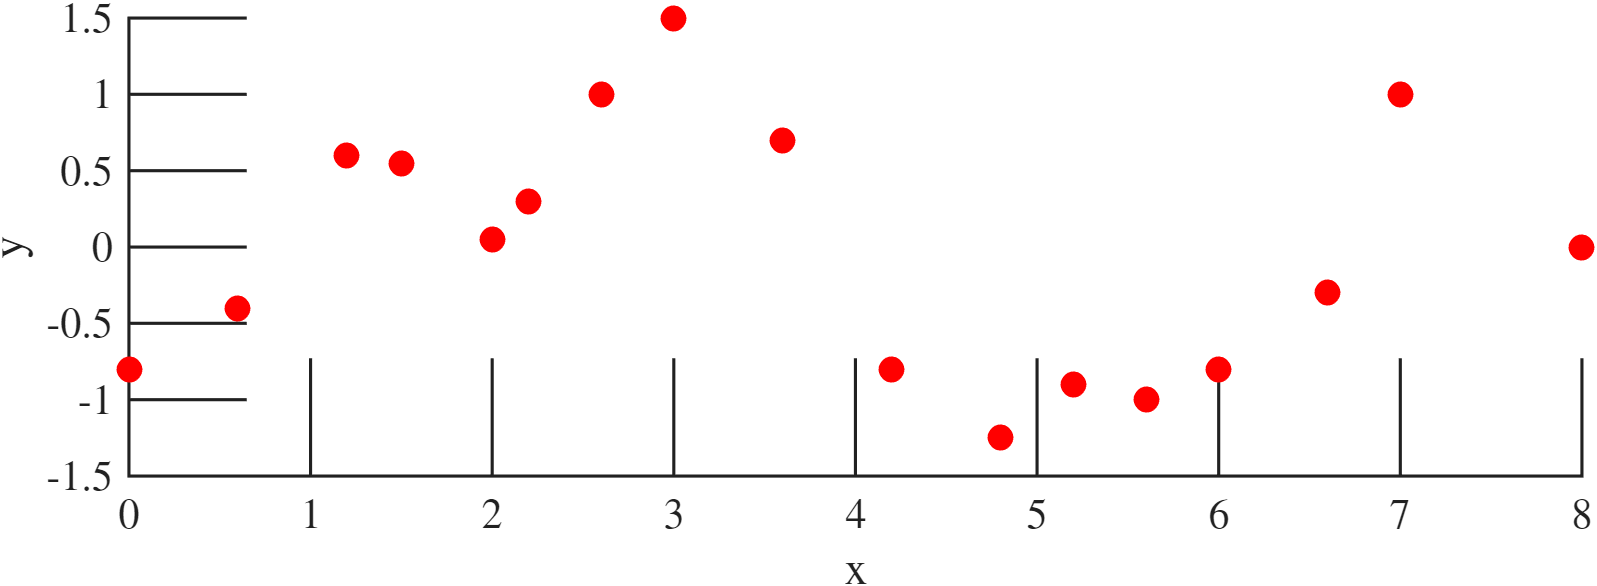
\includegraphics[width=0.6\linewidth]{figs/problem1.png}
\end{figure}
\end{block}

\begin{itemize}
    \item Recall this example 
    \item There are $17$ data points
    \item That means we must fit a degree $sixteen$ polynomial
\end{itemize}
\end{frame}

\begin{frame}{Runge's Phenomenon}

\begin{figure}
    \centering
    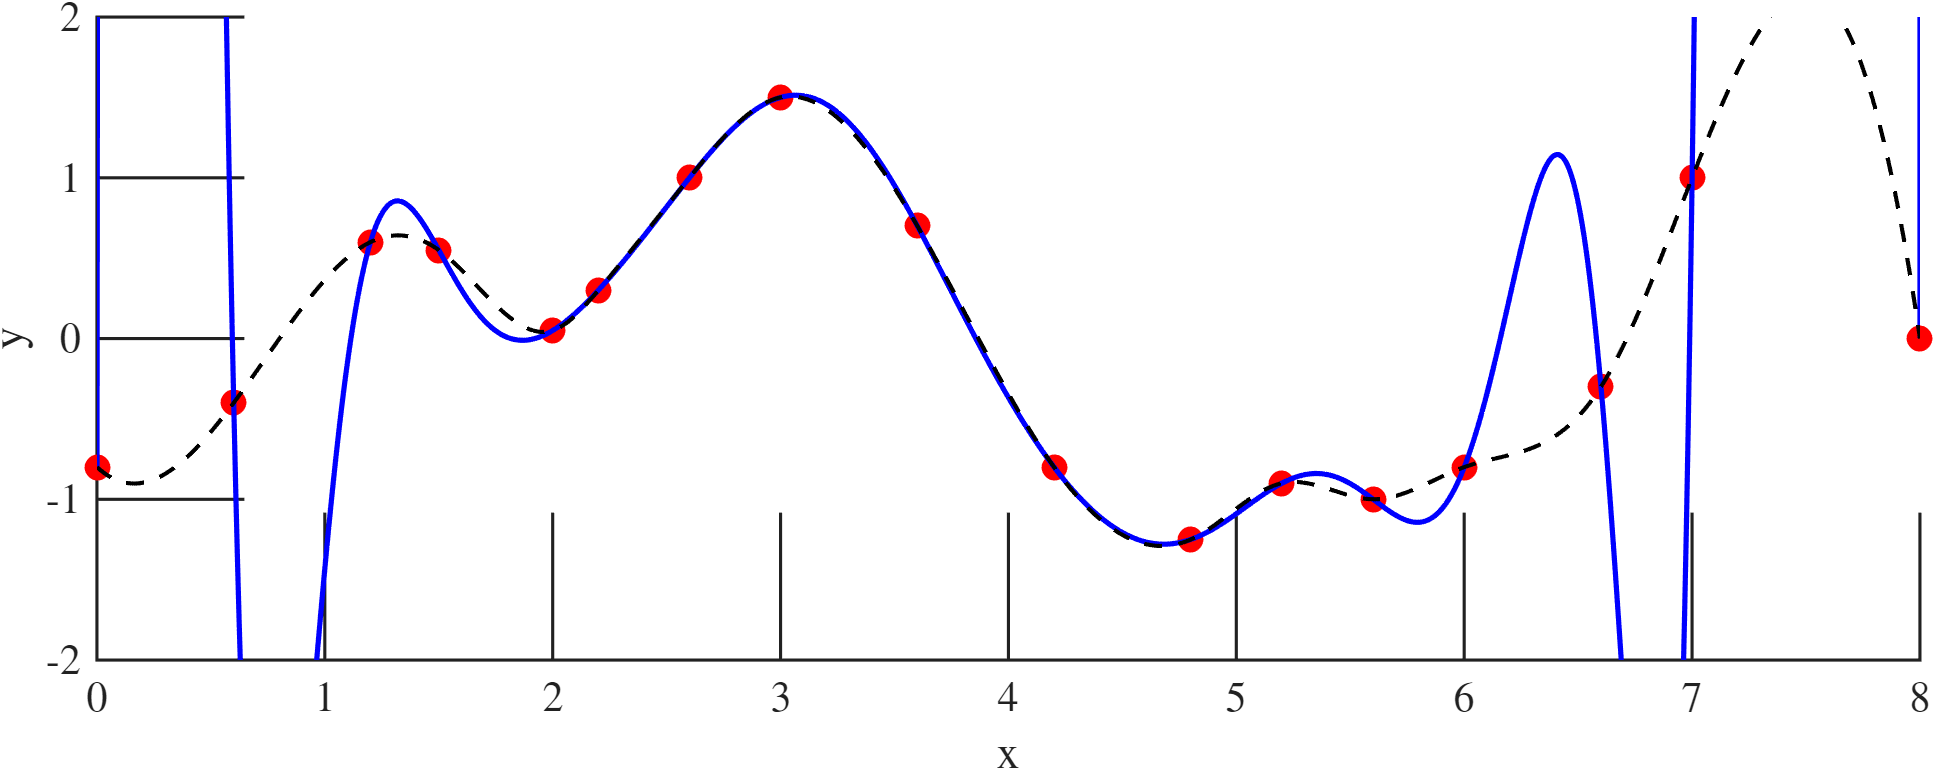
\includegraphics[width=0.9\linewidth]{figs/spline_vs_poly.png}
\end{figure}

\begin{itemize}
    \item Polynomial interpolation plotted in blue has large oscillations near the end
    \item Cubic spline interpolation plotted in dashed lines is well-behaved 
\end{itemize}
\keyidea{
Cubic splines avoid Runge’s phenomenon by using low-degree polynomials locally instead of one high-degree polynomial globally.
}
\end{frame}
%%%%%%%%%%%%%%%%%%%%%%%%%%%%%%%%%%%%%%%%%%%
\sectionframe{3D Data}
%%%%%%%%%%%%%%%%%%%%%%%%%%%%%%%%%%%%%%%%%%%

\begin{frame}[fragile]{3D Data Points}
\begin{itemize} \item 3D data consists of a collection of coordinates
\[
(x_i,y_i,z_i).
\]

\item Example: 25 discrete points on $f(x,y)=x^2+y^2$
\begin{lstlisting}
scatter3(x,y,z)
\end{lstlisting}
\cols{
\begin{figure}
    \centering
    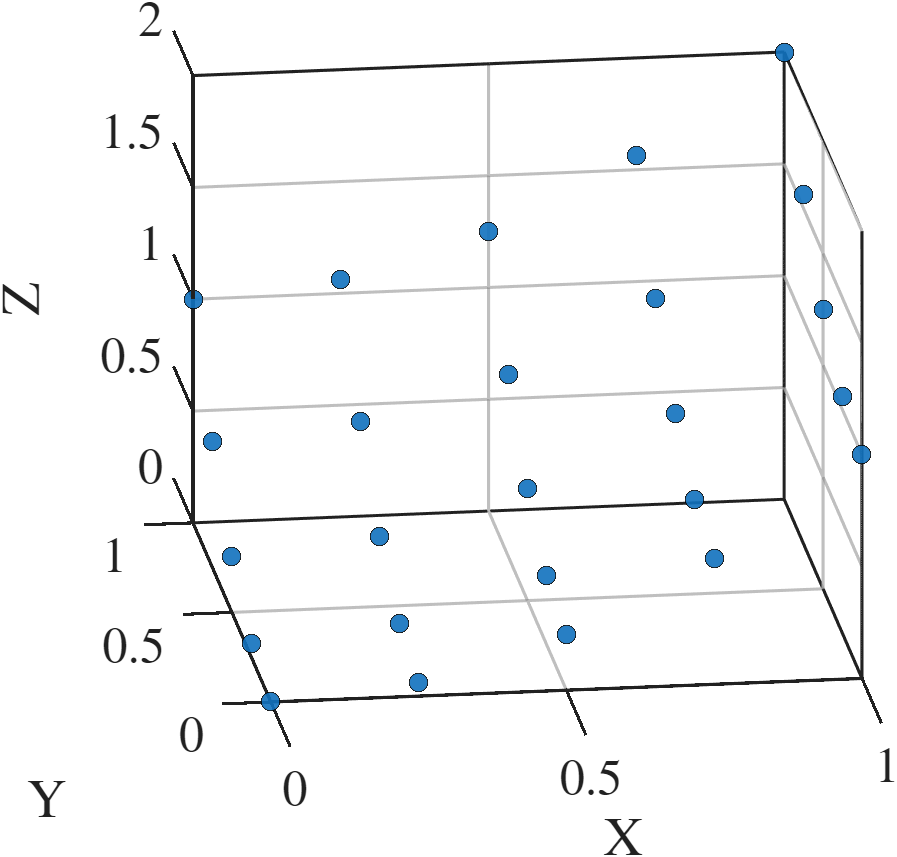
\includegraphics[width=0.9\linewidth]{figs/scatterdata.png}
\end{figure}
}{
    \[
    x=
\begin{bmatrix}
x_1 \\
x_2 \\
\vdots \\
x_n 
\end{bmatrix}
    y=
\begin{bmatrix}
y_1\\
y_2\\
\vdots \\
y_n 
\end{bmatrix}
    z=
\begin{bmatrix}
z_1 \\
z_2 \\
\vdots \\
z_n
\end{bmatrix}
\]
}
\end{itemize} 
\end{frame}


%%%%%%%%%%%%%%%%%%%%%%%%%%%%%%%%%%%%%
\begin{frame}{Face}
\begin{itemize}
    \item A panel created from connecting 4 points is called a \textbf{face}
    \begin{figure}
    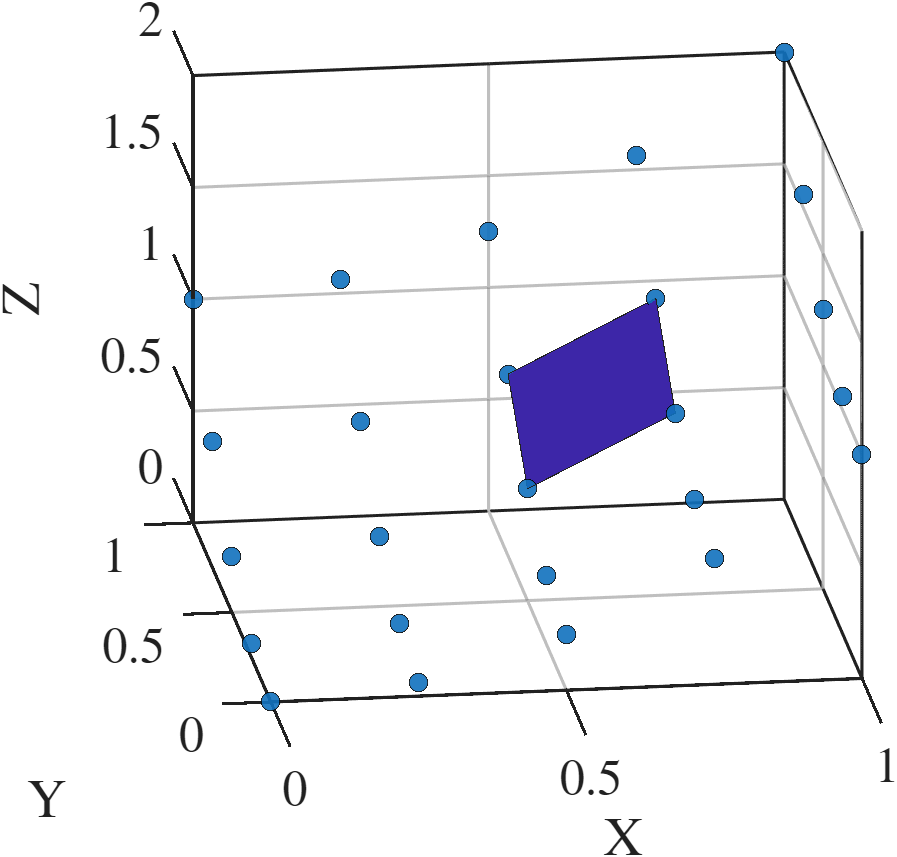
\includegraphics[width=0.4\linewidth]{figs/scatterdata_b.png}
\end{figure}
    \item Plotting all faces creates a surface
\end{itemize}

\question{How can you tell which 4 points form a face?}
\end{frame}

%%%%%%%%%%%%%%%%%%%%%%%%%%%%%%%%%%%%%

\begin{frame}[fragile]{Organizing Surface Data}


\begin{itemize}
    \item This format is not great because we cannot determine faces 
       \[
    x=
\begin{bmatrix}
x_1 \\
x_2 \\
\vdots \\
x_n 
\end{bmatrix}
    y=
\begin{bmatrix}
y_1\\
y_2\\
\vdots \\
y_n 
\end{bmatrix}
    z=
\begin{bmatrix}
z_1 \\
z_2 \\
\vdots \\
z_n
\end{bmatrix}
\]

    \item This format is better because faces are implicit
\[
X=
\begin{bmatrix}
x_{11} & \cdots & x_{1n}\\
\vdots & \ddots & \vdots\\
x_{m1} & \cdots & x_{mn}
\end{bmatrix},
\quad
Y=
\begin{bmatrix}
y_{11} & \cdots & y_{1n}\\
\vdots & \ddots & \vdots\\
y_{m1} & \cdots & y_{mn}
\end{bmatrix},
\quad
Z=
\begin{bmatrix}
z_{11} & \cdots & z_{1n}\\
\vdots & \ddots & \vdots\\
z_{m1} & \cdots & z_{mn}
\end{bmatrix}.
\]
    \item Use \texttt{meshgrid} in matlab
\begin{lstlisting}
x = linspace(0,1,N);
y = linspace(0,1,N);
[X,Y] = meshgrid(x,y);
Z = X.^2 + Y.^2;
\end{lstlisting}

\end{itemize}

\end{frame}

%%%%%%%%%%%%%%%%%%%%%%%%%%%%%%%%%%%%%%%%%%%

\begin{frame}[fragile]{Visualization}

\begin{lstlisting}
x = linspace(0,1,N);
y = linspace(0,1,N);
[X,Y] = meshgrid(x,y); % X and Y are matrices
Z = X.^2 + Y.^2;       % Z is also a matrix
surf(X,Y,Z)
\end{lstlisting}

\cols{
\begin{itemize}
    \item Suppose $X$, $Y$, and $Z$ are matrices housing rectangular grid of coordinates
    \item Function \texttt{surf(X,Y,Z)} plots all faces based on adjacency
\end{itemize}
}{
    \begin{figure}
        \centering
        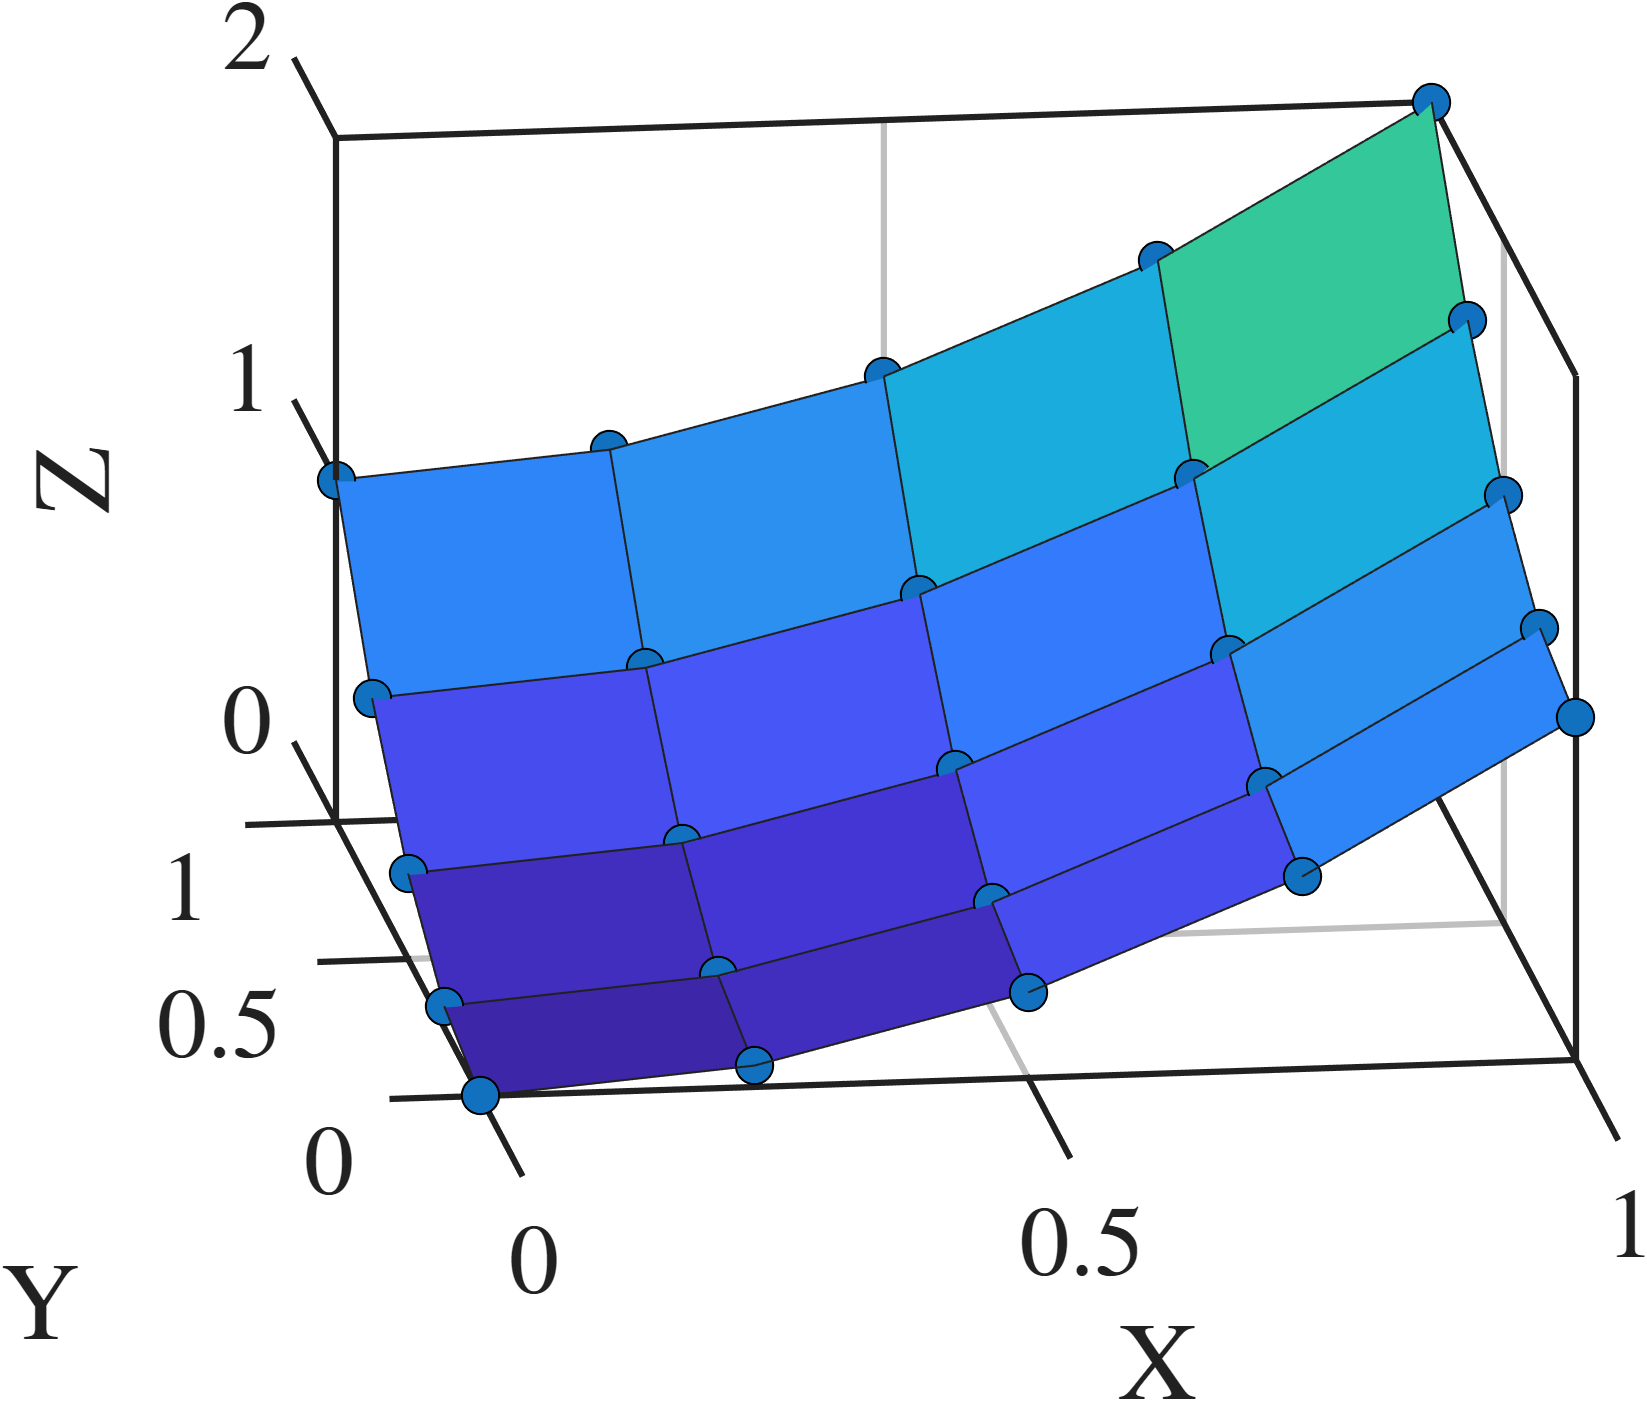
\includegraphics[width=0.9\linewidth]{figs/surf.png}
    \end{figure}
}


\end{frame}

%%%%%%%%%%%%%%%%%%%%%%%%%%%%%%%%%%%%%%%%%%%
\begin{frame}{Function \texttt{interp1()}}
    
\begin{itemize}
    \item You may fit a spline on 3 original data points stored in \texttt{x} and \texttt{y}
\begin{center}
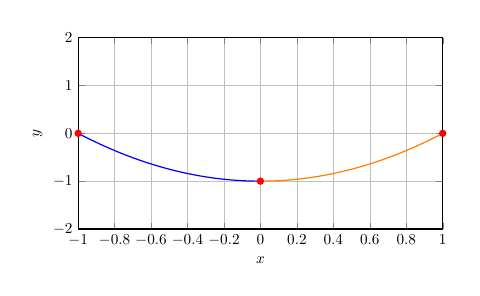
\begin{tikzpicture}[scale=0.55]
    \begin{axis}[
        width=10cm, height=6cm,
        xlabel={$x$}, ylabel={$y$},
        grid=major, 
        thick,
        xmin=-1, xmax=1,
        ymin=-2, ymax=2,
        samples=100,
    ]
    % Quadratic spline segment s0(x) for [-1, 0]
    \addplot[color=blue, thick, domain=-1:0] {x^2-1}; % Example function for s0(x)

    % Quadratic spline segment s1(x) for [0, 1]
    \addplot[color=orange, thick, domain=0:1] {x^2 -1}; % Example function for s1(x)

    % Data points
    \addplot[color=red, only marks, mark=*] 
        coordinates {(-1, 0) (0, -1) (1, 0)};
    \end{axis}
\end{tikzpicture}
\end{center}

    \item Then \texttt{yq = interp1(x,y,xq)} generates extra points $(xq_i,yq_i)$
\begin{center}
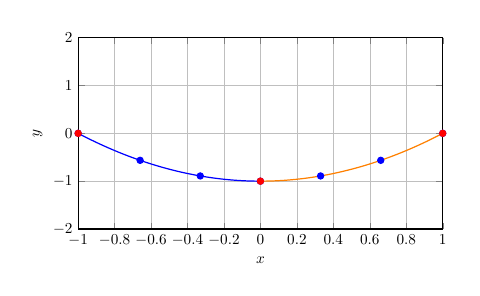
\begin{tikzpicture}[scale=0.55]
    \begin{axis}[
        width=10cm, height=6cm,
        xlabel={$x$}, ylabel={$y$},
        grid=major, 
        thick,
        xmin=-1, xmax=1,
        ymin=-2, ymax=2,
        samples=100,
    ]
    % Quadratic spline segment s0(x) for [-1, 0]
    \addplot[color=blue, thick, domain=-1:0] {x^2-1}; % Example function for s0(x)

    % Quadratic spline segment s1(x) for [0, 1]
    \addplot[color=orange, thick, domain=0:1] {x^2 -1}; % Example function for s1(x)

    % Data points
    \addplot[color=blue, only marks, mark=*] 
        coordinates {(-1, 0) (-0.66, -0.5644) (-0.33,-0.8911)  (0.66, -0.5644) (0.33,-0.8911)(0, -1) (1, 0)};
    \addplot[color=red, only marks, mark=*] 
        coordinates {(-1, 0) (0, -1) (1, 0)};
    
    \end{axis}
\end{tikzpicture}
\end{center}
\end{itemize}
\end{frame}

%%%%%%%%%%%%%%%%%%%%%%%%%%%%%%%%%%%%%%%%%%%

\begin{frame}[fragile]{Function \texttt{interp2()}}

\begin{itemize}
    \item The function \texttt{interp2} works the same way with matrices

\begin{lstlisting}
level = 1;
Xq = interp2(X,level,'spline');
Yq = interp2(Y,level,'spline');
Zq = interp2(Z,level,'spline');
mesh(Xq,Yq,Zq)
\end{lstlisting}

    \item Parameter \texttt{level} controls the refinement

\begin{figure}
    \centering
    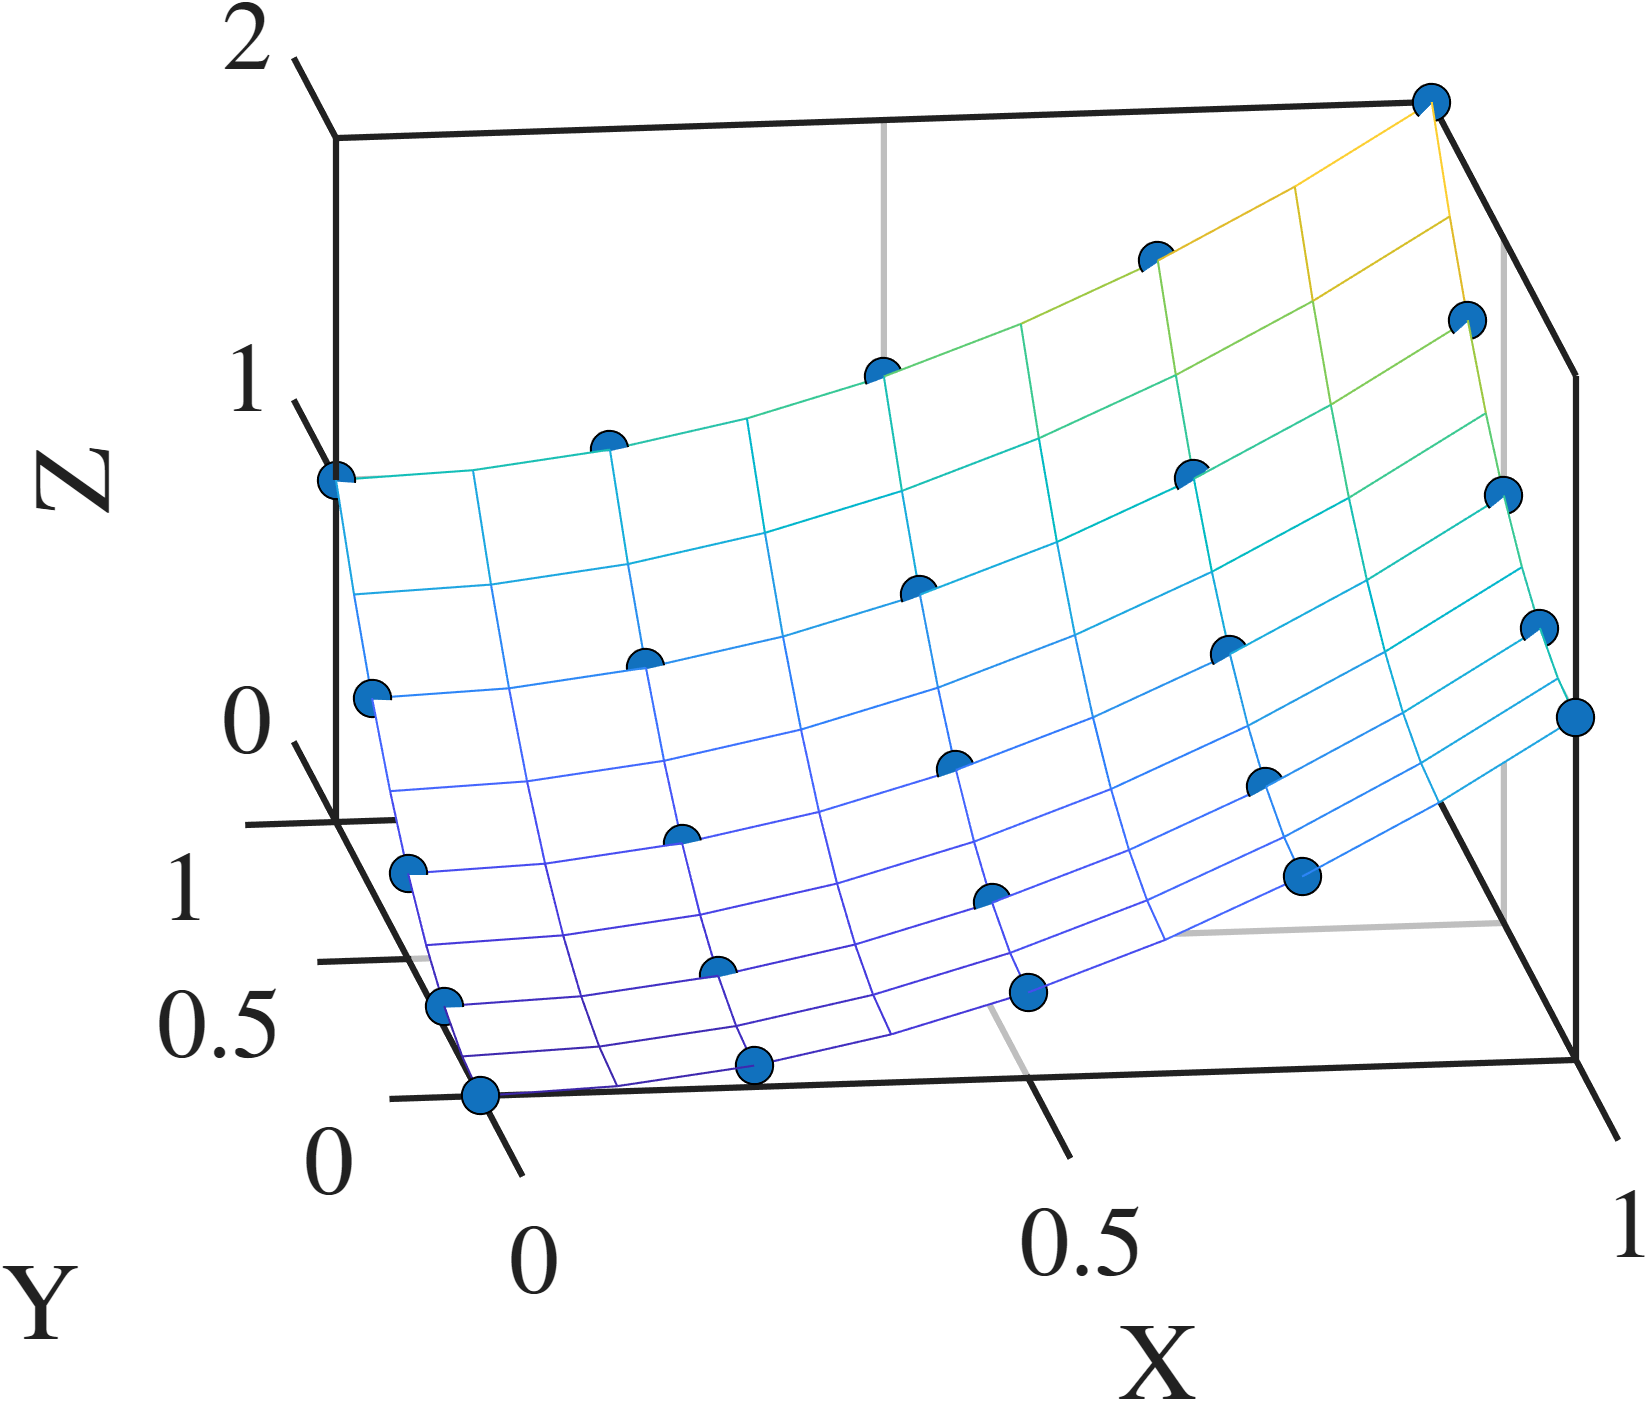
\includegraphics[width=0.45\linewidth]{figs/interp2a.png}
    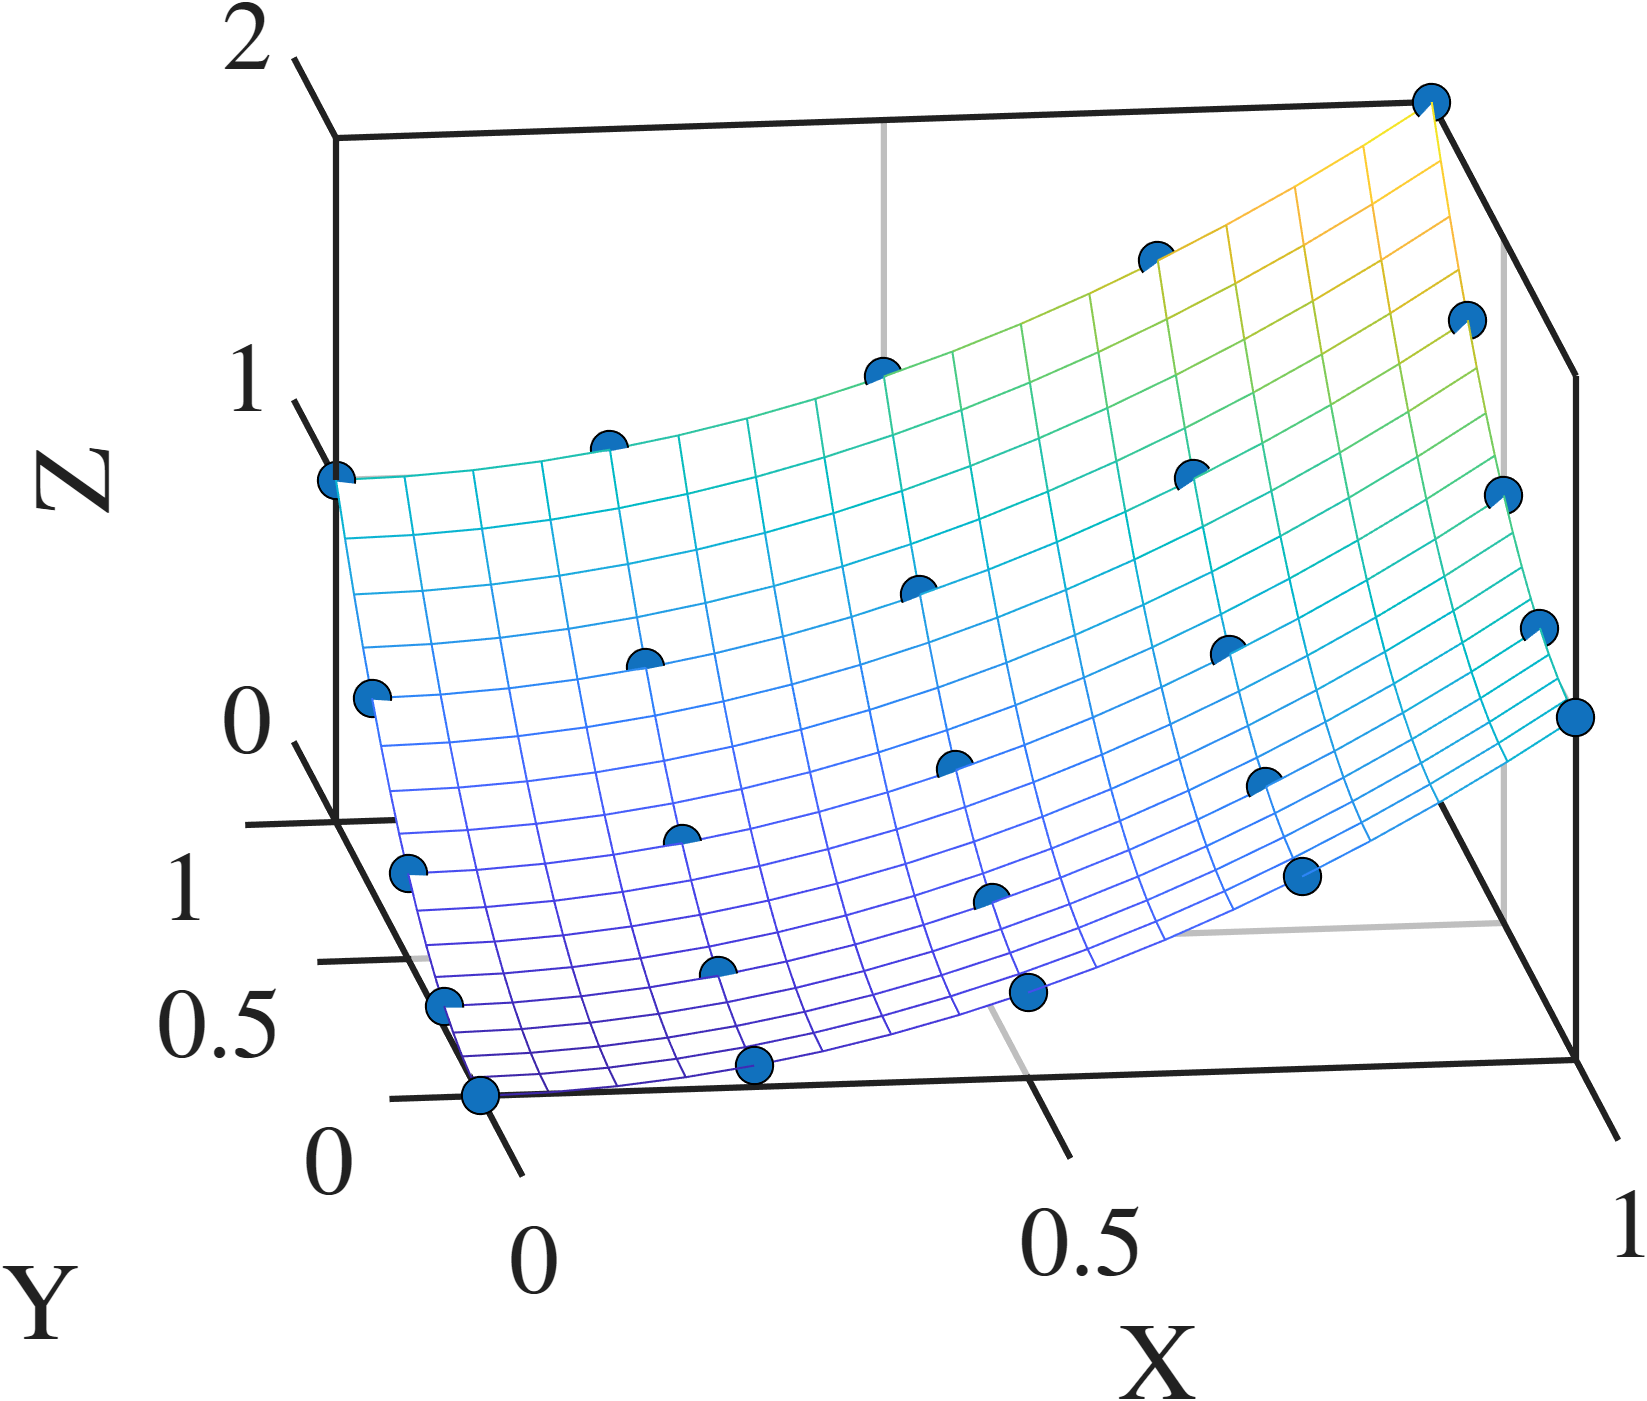
\includegraphics[width=0.45\linewidth]{figs/interp2b.png}
\end{figure}




\end{itemize}
\end{frame}

%%%%%%%%%%%%%%%%%%%%%%%%%%%%%%%%%%%%%%%%%%%

\begin{frame}[fragile]{Building an Object from Patches}

\cols{
\begin{itemize}
    \item  A general object can contain multiple surfaces
    \item Each half is called a \textbf{patch}
    \item Access patch with last index 
    $$
    X(:,:,k), \; Y(:,:,k), \; Z(:,:,k)
    $$
    
\end{itemize}
}{
\begin{figure}
    \centering
    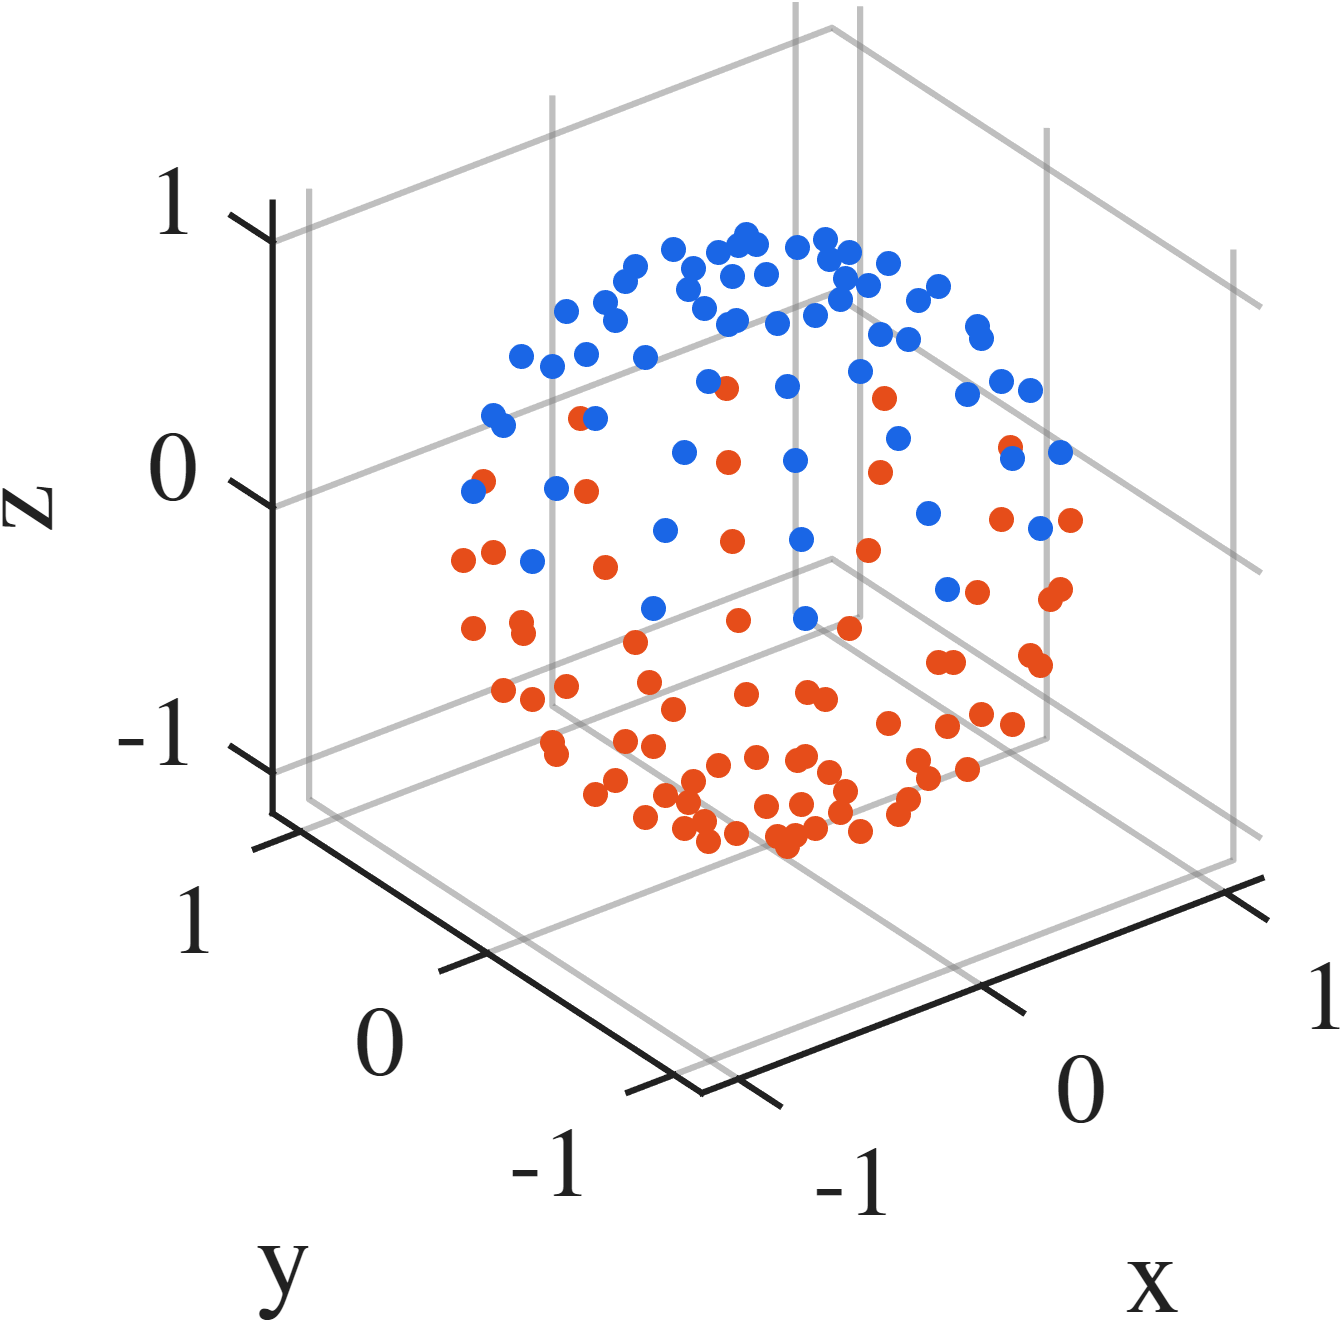
\includegraphics[width=0.9\linewidth]{figs/sphere_patch.png}
\end{figure}
}
\begin{lstlisting}
X(:,:,1), Y(:,:,1), Z(:,:,1) % top half of sphere 
X(:,:,2), Y(:,:,2), Z(:,:,2) % bottom half 
\end{lstlisting}

\end{frame}

%%%%%%%%%%%%%%%%%%%%%%%%%%%%%%%%%%%%%%%%%%%
\begin{frame}{Interpolated Sphere}
\cols{
    \begin{itemize}
        \item Interpolate each patch with \texttt{interp2}
        \item Plot the surface of each interpolation with \texttt{surf}
    \end{itemize}
}{
\begin{figure}
    \centering
    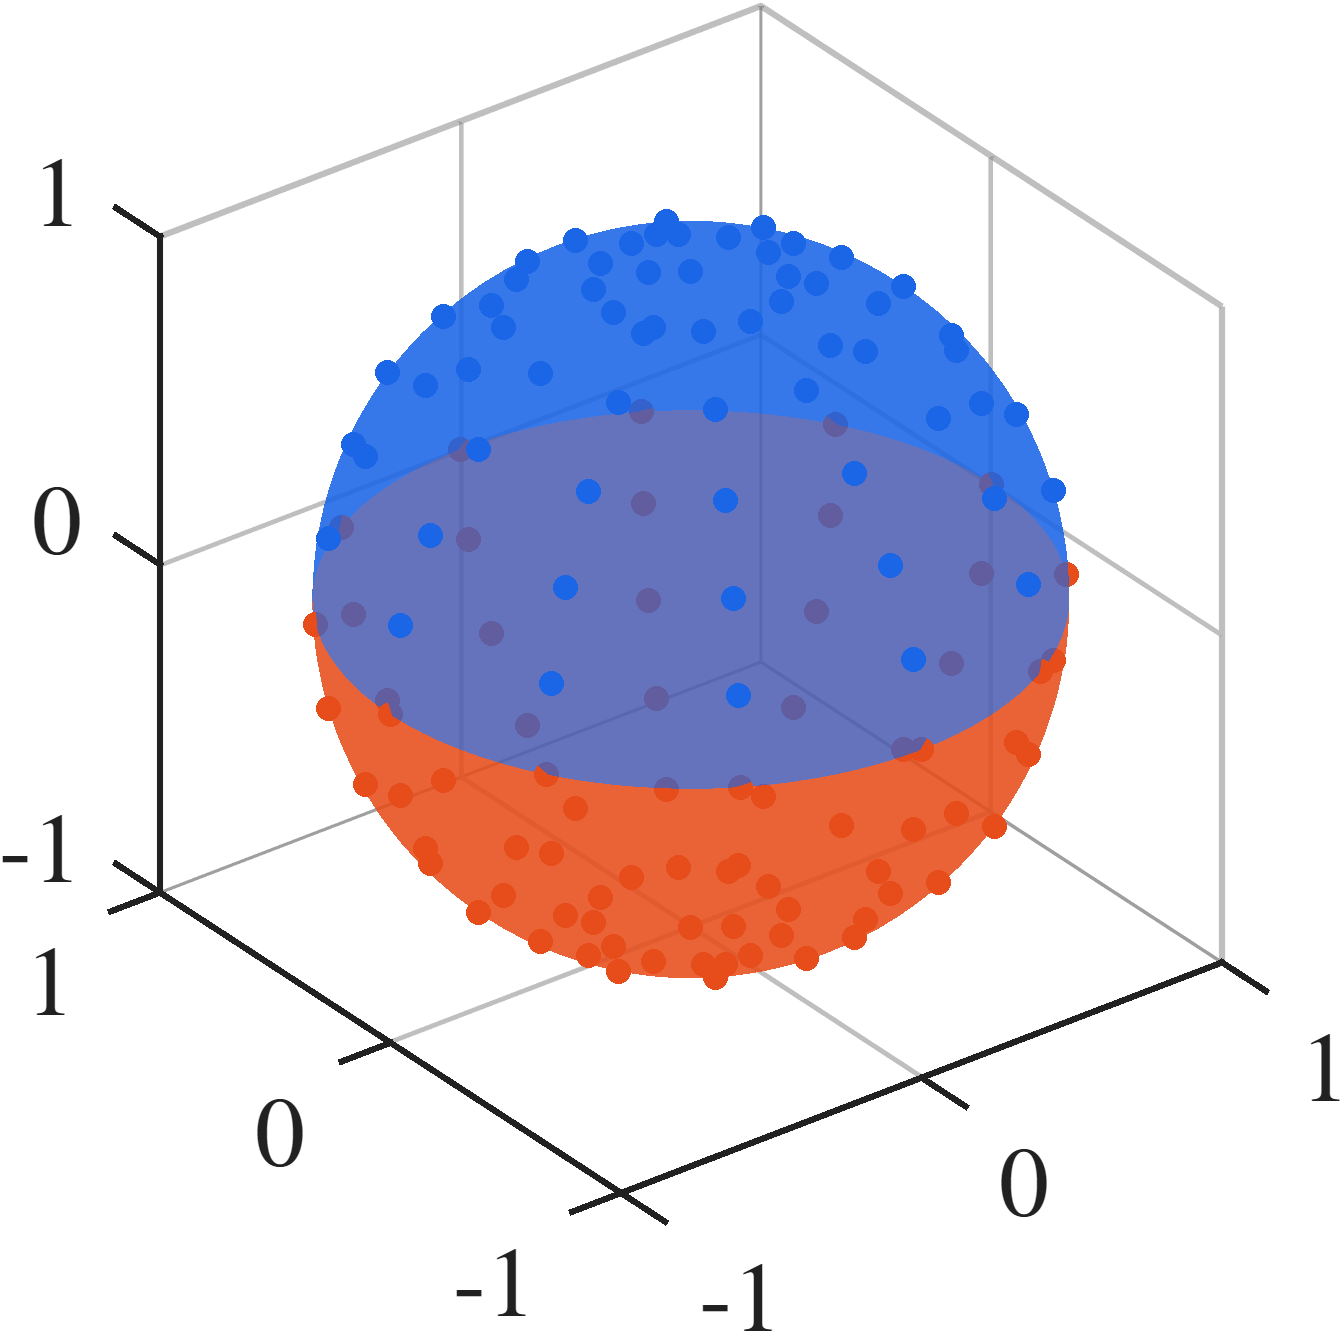
\includegraphics[width=0.9\linewidth]{figs/sphere_interp.png}
\end{figure}

}
\end{frame}
%%%%%%%%%%%%%%%%%%%%%%%%%%%%%%%%%%%%%%%%%%%

\begin{frame}[fragile]{Finishing Touches}

\begin{lstlisting}
shading interp
colormap copper
axis equal
axis off
view(135,25)
camlight headlight
lighting gouraud
\end{lstlisting}

\begin{figure}
    \centering
    
\includegraphics[width=0.4\linewidth]{figs/sphere_complete.png}
\end{figure}

\end{frame}

\end{document}



